\documentclass[../../main.tex]{subfiles}
\begin{document}
%
\section{Gaussian Chain}\label{ch: Gaussian Chain}
    
    The study of polymers in solution can start with an investigation on the dynamics of a single polymer chain in two dimensions. This simple case corresponds to the limit of diluted solution, where interactions between different polymers chains are negligible. 
    
    From a physical standpoint, a polymer can be thought as a set of $N+1$ connected monomers forming a chain. The corresponding bond vectors are defined as
        \begin{equation}\label{eq: Gaussian Chain - Bond Vector Definition}
            \{\mathbf{r}_n\}\equiv(\mathbf{r}_1, \,\ldots,\, \mathbf{r}_N) \,,
        \end{equation}
    with $\mathbf{r}_n = \mathbf{R}_n - \mathbf{R}_{n-1}$, of which $\{\mathbf{R}_n\} \equiv (\mathbf{R}_0, \,\ldots,\, \mathbf{R}_N)$ are the position vectors for all monomers.
    
    In our model, the bond vectors are independent of each other, making it possible for a bond to be oriented in every direction, irrespective of the orientation of the others. Accordingly, we allow for the beads, and respective bonds to cross without penalty. The distribution function of the polymer conformation will then be given by
        \begin{equation}\label{eq: Gaussian Chain - Distribution function of the polymer conformation (I)}
            \Psi(\{\mathbf{r}_n\}) = \prod_{n=1}^N \psi(\mathbf{r}_n) \,,
        \end{equation}
   % where $...$ [Phi x dr] is the probability that the bond vector for the bond $n$ is $r_n$. In the limit of rigid bonds of length $b$,   
    where $\psi(\mathbf{r}_n)$ is the normalised distribution of a bond vector
        \begin{equation}\label{eq: Gaussian Chain - Normalised distribution of a random bond vector}
            \psi(\mathbf{r_n}) = \frac{1}{2\pi b}\delta(\lvert\mathbf{r}_n\rvert - b) \,,
        \end{equation}
    with $b$ being the effective bond length, that we assume to be the same for all bonds. %This parameter defines the minimum length between two uncorrelated points in the polymer chain, and can offer a sense of the "stiffness" of the chain, here on quotation marks since, strictly speaking, this model does not account for stiffness. Nevertheless, we can note that a smaller $b$ might correspond to a greater number of degrees of freedom, and thus be characteristic of a more flexible chain, with the opposite being also true. 

    Instead of working with all the possible conformations that our polymer chain can have, it becomes more convenient to describe it by its end-to-end vector, $\mathbf{B}$. 
    
    $\mathbf{B}$ is a measure of the chain size, that can be easily found experimentally through light scattering techniques. Conversely to the more conventional case, where thermodynamic quantities are expected to show some proportionality to the number of elements, the size of a polymer chain, in thermal equilibrium, yields a different dependence. How the size of a polymer scales as its length is increased, whether it shows a dependence on the temperature or on any other internal or external parameter to the chain, all form interesting questions. 
    
    Let the probability distribution function for $\mathbf{B}$ be given by
        \begin{equation}\label{eq: Gaussian Chain - PDF of the e2e vector of a chain - I}
            \Phi(\mathbf{B}) = \bigintsss \ldots \bigintsss_N \delta\left( \mathbf{B} - \sum_{n = 1}^N \mathbf{r}_n \right) \Psi(\{\mathbf{r}_n\}) \, d\mathbf{r}_1 \ldots d\mathbf{r}_n \,.
        \end{equation}
    Using,
        \begin{equation}\label{eq: Gaussian Chain - Delta Kronecker}
            \delta (\mathbf{r}) = \frac{1}{(2\pi)^2}\bigintssss \exp(i\mathbf{k}\cdot \mathbf{r}) d\mathbf{k} \,,
        \end{equation}
    and with $\Psi(\{\mathbf{r}_n\})$ given by \cref{eq: Gaussian Chain - Distribution function of the polymer conformation (I)}, we obtain
        \begin{equation}\label{eq: Gaussian Chain - PDF of the e2e vector of a chain - II}
        \begin{split}
            \Phi(\mathbf{B}) &= 
            \frac{1}{(2\pi)^2} \bigintssss \exp\left( i\mathbf{k}\cdot \mathbf{B} \right) d\mathbf{k} \bigintssss_N \prod_{n = 1}^N \exp \left(-i\mathbf{k}\cdot\mathbf{r}_n\right)\psi(\mathbf{r_n}) d^n\mathbf{r} = \\
            &= \frac{1}{(2\pi)^2} \bigintssss \exp\left( i\mathbf{k}\cdot \mathbf{B} \right) d\mathbf{k} \left[\bigintssss \exp\left(- i\mathbf{k}\cdot\mathbf{r} \right)\psi(\mathbf{r}) d\mathbf{r}\right]^N \,.
        \end{split}
        \end{equation}
        
    The portion of \cref{eq: Gaussian Chain - PDF of the e2e vector of a chain - II} that consists of the integral over $\mathbf{r}$ can be evaluated by introducing polar coordinates
        \begin{equation}
            \frac{1}{2\pi b} \bigintssss_0^\infty r dr \bigintssss_0^{2\pi}\exp\left[ -ikr\cos(\phi)\right]\delta\left(r-b\right) d\phi = J_0(kb) \,,
        \end{equation}
     where $k = \lvert \mathbf{k} \lvert$ and $J_0(kb)$ is the Bessel function of the first kind. We consider $N$ to be large, and perform a Taylor expansion of the Bessel function, which leads to
        \begin{equation}\label{eq: Gaussian Chain - approx of the sin^N}
            \left( 1-\frac{(kb)^2}{4}\right)^N \approx \exp \left(-\frac{Nk^2b^2}{4}\right) \,,
        \end{equation}
    allowing us to write \cref{eq: Gaussian Chain - PDF of the e2e vector of a chain - II} as
        \begin{equation}\label{eq: Gaussian Chain - PDF of the e2e vector of a chain - III}
             \Phi(\mathbf{B}) = \frac{1}{(2\pi)^2} \bigintssss \exp\left( i\mathbf{k}\cdot \mathbf{B} - \frac{N\mathbf{k}^2b^2}{4} \right) d\mathbf{k} \,.
        \end{equation}
        
    This is a Gaussian integral that can be easily solved (\cref{app: Gaussian Int}). Taking $k_\alpha$ and $B_\alpha$, where $\alpha$ denotes the components of the vectors $\mathbf{k}$ and $\mathbf{B}$, we get 
        \begin{equation}\label{eq: Gaussian Chain - PDF of the e2e vector of a chain - IV}
        \begin{split}
            \Phi(\mathbf{B}) &= \frac{1}{(2\pi)^2} \prod_\alpha \left[\bigintssss_{-\infty}^\infty \exp\left( ik_\alpha\cdot B_\alpha - \frac{Nk_\alpha^2b^2}{4} \right) dk_\alpha \right] = \\
            %&= \frac{1}{(2\pi)^2} \prod_\alpha\left[ \sqrt{\frac{4\pi}{Nb^2}}\exp\left( -\frac{1}{Nb^2}B_\alpha^2 \right) \right] = \\
            %&= \frac{1}{(2\pi)^2}\frac{4\pi}{Nb^2}\exp\left( -\frac{\mathbf{B}^2}{Nb^2}\right) = \\
            &= \frac{1}{\pi Nb^2} \exp\left( -\frac{\mathbf{B}^2}{Nb^2} \right) \,.
        \end{split}
        \end{equation}
    
    The approximation of the distribution function $\Phi(\mathbf{B})$ by \cref{eq: Gaussian Chain - PDF of the e2e vector of a chain - IV} is what we call the Gaussian Chain. So, we consider a chain whose bond length probability, $\psi(\mathbf{r}_n)$, is a Gaussian distribution given by
        \begin{equation}\label{eq: Gaussian Chain - Distribution of a random bond vector}
           \psi(\mathbf{r}_n) = \frac{1}{2\pi b^2} \exp\left( -\frac{\mathbf{r}^2}{b^2} \right) \,,
        \end{equation}
    so that
        \begin{equation}
            \langle \mathbf{r}^2 \rangle = b^2 \,.
        \end{equation}
        
    The distribution function of the end-to-end vector is the Gaussian function given in \cref{eq: Gaussian Chain - PDF of the e2e vector of a chain - IV}. This implies that, in the statistics of the Gaussian Chain, the exact bond probability can be replaced by the Gaussian bond probability. As per \cref{eq: Gaussian Chain - Distribution function of the polymer conformation (I)}, the conformational distribution function of such a chain will be given by
        \begin{equation}\label{eq: Gaussian Chain - Distribution function of the polymer conformation (II)}
        \begin{split}
            \Psi(\{\mathbf{r}_n\}) &= \prod_{n = 1}^N\left[\frac{1}{2\pi b^2} \exp\left( -\frac{\mathbf{r}_n^2}{b^2} \right)\right] =\\
            &= \left( \frac{1}{2\pi b^2} \right)^{N} \exp\left[ -\sum_{n=1}^N \frac{1}{b^2} \left(\mathbf{R}_n-\mathbf{R}_{n-1}\right)^2 \right] \,.
        \end{split}
        \end{equation}
    An important property of this model will be that the distribution of the vector $\mathbf{R}_n - \mathbf{R}_m$, where $n$ and $m$ are any two monomers of our chain, is Gaussian and given by
        \begin{equation}\label{eq: Gaussian Chain - PDF of some vector of the chain}
            \Phi(\mathbf{R}_n - \mathbf{R}_m, n-m) = \frac{\lvert n-m \rvert}{2\pi b^2} \exp\left[ -\frac{\left(\mathbf{R}_n-\mathbf{R}_{n-1}\right)^2}{b^2\lvert n-m \rvert} \right] \,,
        \end{equation}
    and thus
        \begin{equation}\label{eq: Gaussian Chain - Distance between monomers}
            \langle (\mathbf{R}_n - \mathbf{R}_m)^2 \rangle = \lvert n-m \rvert b^2 \,.
        \end{equation}
    If we consider the end-to-end vector of a chain with $N$ links to be $\mathbf{B} = \mathbf{R}_N - \mathbf{R}_0$, then \cref{eq: Gaussian Chain - Distance between monomers} becomes
        \begin{equation}
            \langle \mathbf{B}^2 \rangle = N b^2 \,.
        \end{equation}
    
    So far, we considered stiff bonds of fixed length $b$. We now consider the case where bonds are flexible, with an elastic energy given by
        \begin{equation}\label{eq: Gaussian Chain - Harmonic Spring Potential}
            U_{\kappa_s}(\{\mathbf{r}_n\}) = \frac{\kappa_s}{2}\sum_{n=1}^N \mathbf{r}_n^2, \; \kappa_s = \frac{k_bT}{b^2} \,.
        \end{equation}
    Such equivalence can be easily shown. Since we know the distribution function for a single element to be Boltzmann weighted, it follows that
        \begin{equation}
            \psi(\mathbf{\mathbf{r}_n}) \propto \exp \left(-\frac{U_{\kappa_s}}{k_BT}\right) = \exp \left(-\frac{\mathbf{r}_n^2}{2b^2}\right) \,,
        \end{equation}
    leaving only the normalisation constant, $c$, to be calculated. Given 
        \begin{equation}\label{eq: Gaussian Chain - Normalization Integral}
            \bigintssss \psi(\mathbf{r}_n) d\mathbf{r}_n = 1 \,,
        \end{equation}
    the right-hand side can be simplified as,
        \begin{equation}
            c \bigintssss_0^{2\pi} d\phi \bigintssss_0^\infty r_n\exp\left(-\frac{r_n^2}{2b^2}\right) = 2\pi c b^2 \,,
        \end{equation}
    and so
        \begin{equation}
            c = \frac{1}{2\pi b^2} \,,
        \end{equation}
    meaning that, at equilibrium, we recover the result given by \cref{eq: Gaussian Chain - Distribution of a random bond vector}.
    
\subsection{Two-Monomer Chain}\label{subSection: The 2 Monomer Chain}
    Consider a Gaussian chain with two monomers, where the motion for each monomer is determined by the following Langevin equations
        \begin{align}
            \label{eq: Case for 2 Monomers - langevin for the monomer [1]}
            \zeta \frac{d\mathbf{R}_0}{dt} &= -\frac{\partial  U_{\kappa_s}(\{\mathbf{r}_1\})}{\partial \mathbf{R}_0} + \bm{\xi}_0 = \kappa_s \left( \mathbf{R}_1 - \mathbf{R}_0 \right) + \bm{\xi}_0 \,,\\
            \label{eq: Case for 2 Monomers - langevin for the monomer [2]}
            \zeta \frac{d\mathbf{R}_1}{dt} &= -\frac{\partial  U_{\kappa_s}(\{\mathbf{r}_1\})}{\partial \mathbf{R}_1} + \bm{\xi}_1 = -\kappa_s \left( \mathbf{R}_1 - \mathbf{R}_0 \right) + \bm{\xi}_1 \,. 
        \end{align}
    
    Using the bond vector definition, we can rewrite \cref{eq: Case for 2 Monomers - langevin for the monomer [1],eq: Case for 2 Monomers - langevin for the monomer [2]} as
        \begin{equation}\label{eq: Case for 2 Monomers - langevin for the bond}
            \zeta \frac{d\mathbf{r}}{dt} = -2\kappa_s\mathbf{r} + \bm{\Xi} \,,
        \end{equation}
    where $\bm{\Xi} = \bm{\xi}_1 -  \bm{\xi}_0$, meaning that
        \begin{align}
            \left\langle \bm{\Xi} \right\rangle &= 0 \,,\\
            \left\langle \Xi_{\alpha_1}(t_1) \Xi_{\alpha_2}(t_2) \right\rangle &= 2g \delta_{{\alpha_1}{\alpha_2}} \delta(t_1 - t_2)\,.
        \end{align}
    
    To get the position correlation function, we take \cref{eq: Case for 2 Monomers - langevin for the bond} and express $\mathbf{r}$ in terms of $\bm{\Xi}$ (see \cref{app: 1st ODE})
        \begin{equation}
            \mathbf{r}(t) = \frac{1}{\zeta}\bigintsss_0^t \bm{\Xi}(t_1) \exp\left(-\frac{t-t_1}{\tau}\right)dt_1 \,,
        \end{equation}
    where $\tau = \zeta/2\kappa_s$. Hence
        \begin{equation}\label{eq: Case for 2 Monomers - pos corr (theory)}
        \begin{split}
            \langle \mathbf{r}^2(t) \rangle &= \frac{1}{\zeta^2}\bigintsss_0^t \bigintsss_0^t \left\langle \bm{\Xi}(t_1) \cdot \bm{\Xi}(t_2) \right\rangle \exp\left( -\frac{t-t_1}{\tau} \right) \exp\left( -\frac{t-t_2}{\tau} \right) dt_1dt_2 = \\
            &= \frac{d_s g}{2\zeta\kappa_s} \left[1 - \exp\left( -\frac{4\kappa_s}{\zeta}t \right)\right]\,.
        \end{split}
        \end{equation}
    
    The position correlation function can not only offer some insight on the system in question but, with a straightforward implementation, it can also be used as a way to validate our code. By tracking the motion of a large number of particle pairs, we have that their average position, $\langle \mathbf{r}(t) \rangle$, at time $t$ is given by
        \begin{equation}
            \langle \mathbf{r}(t) \rangle = \frac{1}{N} \sum_{n = 0}^N \mathbf{r}_n(t) \,,
        \end{equation}
    where $\mathbf{r}_n(t)$ is the position vector of the $n$-th particle pair at time $t$. It follows that the position correlation function is given by
        \begin{equation}\label{eq: Case for 2 Monomers - pos corr (num)}
            \langle \mathbf{r}^2(t) \rangle = \frac{1}{N} \sum_{n = 0}^N \mathbf{r}_n^2(t) \,.
        \end{equation}
        \begin{figure}[h]
            \centering
            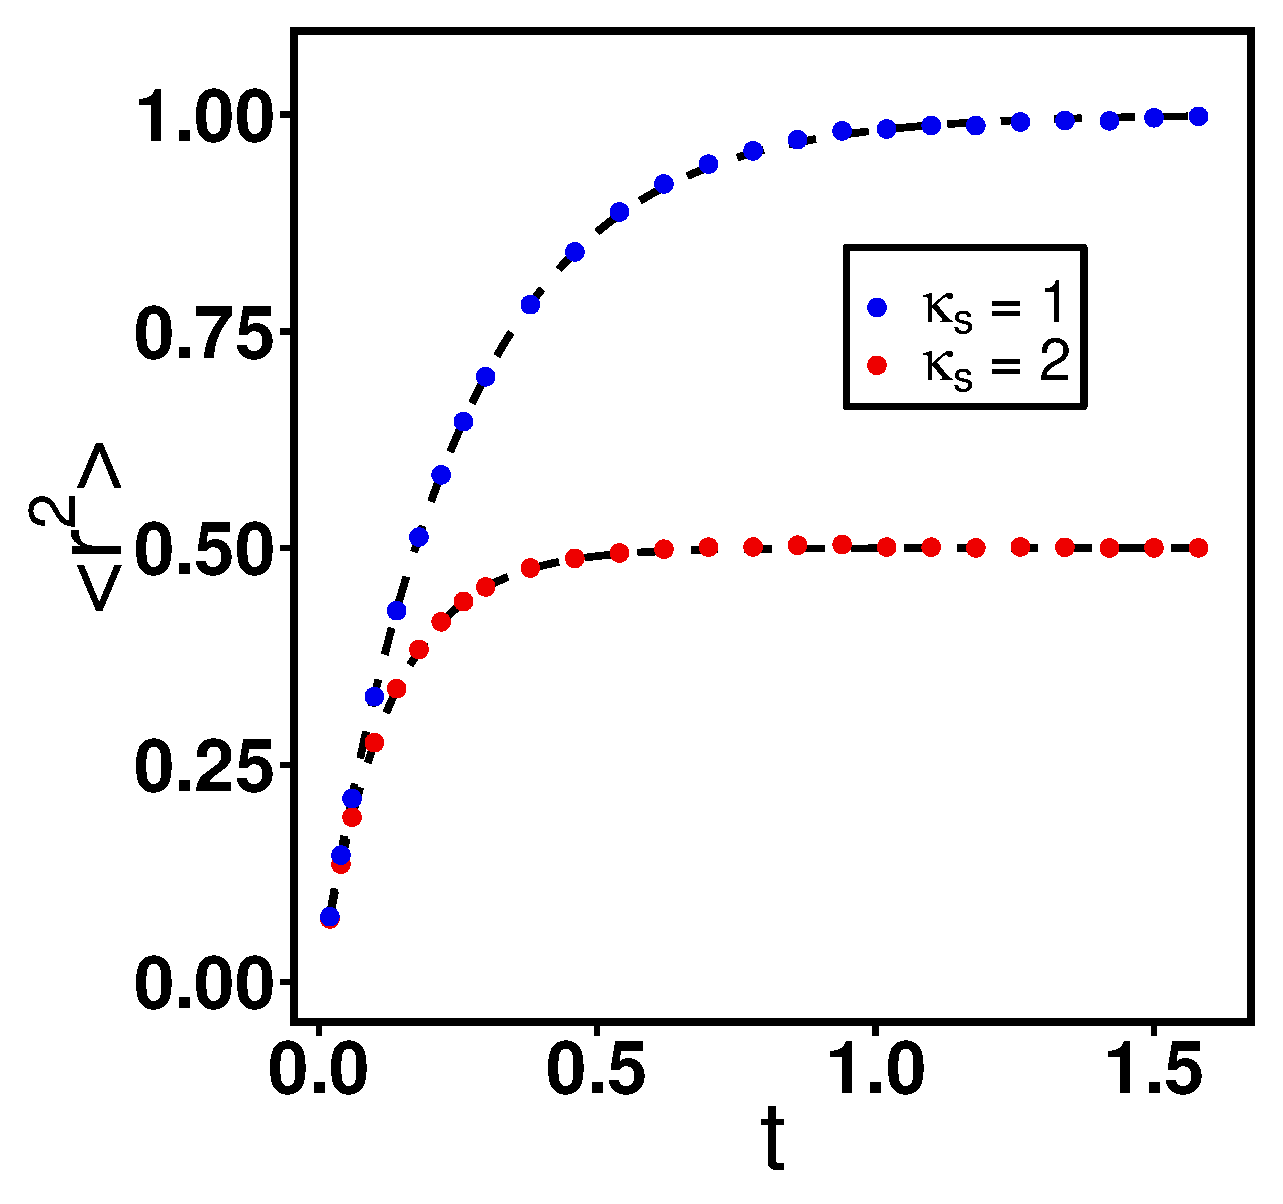
\includegraphics[scale=0.4]{Figures/mon2.eps}
            \caption{ With \cref{eq: Case for 2 Monomers - pos corr (num)} we are capable of calculating the position correlation of our two-monomer chain to which we can compare to \cref{eq: Case for 2 Monomers - pos corr (theory)}, represented by the dashed line. Both methods produce the same result meaning that our code is validated. Parameters used: $g = 1$.}
            \label{fig: 2mon chain}
        \end{figure}
   
    We show in \cref{fig: 2mon chain} that \cref{eq: Case for 2 Monomers - pos corr (num)} is equivalent to \cref{eq: Case for 2 Monomers - pos corr (theory)}. This is the first step towards validating our computational model, be it the use of the integration method or the truncation of the normal distribution function (see \cref{app: Integration Method,app: Dist Trunc}).
    
%\subsection{Viscoelasticity}
\section{Viscoelasticity}
%
    Polymer solutions have interesting mechanical properties exhibiting both viscous and elastic behaviour and thus being viscoelastic. How those phenomena can be understood from the microscopic characteristic of the materials, their structure and the type of interactions, has been a fundamental question in rheology.
%
%\subsubsection{2-monomer chain: stress tensor and viscosity}
\subsection{Two-Monomer Chain: Stress Tensor and Viscosity}
%
    Suppose that we have a shear flow whose velocity field is given by
        \begin{equation}
            \mathbf{u}(x, y) = \Dot{\gamma} y \,\uvec{i} \,,
        \end{equation}
    where $\Dot{\gamma}$ is the shear rate. 
    
    The motion of the particle pair will be given by
        \begin{equation}\label{eq: Case for 2 Monomers - langevin bond with shear}
            \zeta \frac{d\mathbf{r}}{dt} = \zeta \Dot{\gamma} r_y \,\uvec{i} -2\kappa_s\mathbf{r} + \bm{\Xi} \,,
        \end{equation}
    where $r_y$ is the $y$-component of the vector $\mathbf{r}$. Splitting \cref{eq: Case for 2 Monomers - langevin bond with shear} into its components we get the following set of equations
        \begin{equation}\label{eq: Case for 2 Monomers - langevin bond with shear (components)}
            \begin{split}
                \zeta \frac{dr_x}{dt} &= \zeta \Dot{\gamma} r_y -2\kappa_s r_x + \Xi_x \,, \\
                \zeta \frac{dr_y}{dt} &= -2\kappa_s r_y + \Xi_y \,,
            \end{split}
        \end{equation}
    whose solutions, following the steps laid out in \cref{app: 1st ODE}, are
        \begin{equation}\label{eq: Case for 2 Monomers - langevin bond with shear solution}
            \begin{split}
                r_x(t) &= \exp\left(-\frac{t}{\tau}\right) \left[ \bigintss_0^t \left( \Dot{\gamma}r_y(t_1) + \frac{1}{\zeta}\Xi_x(t_1) \right) \exp\left(\frac{t_1}{\tau} \right) dt_1 \right] \,, \\
                r_y(t) &= \exp\left(-\frac{t}{\tau}\right) \left( \frac{1}{\zeta} \bigintss_0^t \Xi_y(t_1) \exp\left(\frac{t_1}{\tau} \right) dt_1 \right) \,.
            \end{split}
        \end{equation}
    
    To obtain the effective viscosity of the fluid, we have to determine the stress tensor of the fluid under shear which is obtained through the general expression
        \begin{equation}
            \sigma_{xy} = \sigma^{(s)}_{xy} + \sigma^{(p)}_{xy} \,,
        \end{equation}
    where $\sigma^{(s)}_{xy}$ is the stress tensor due to the solvent and $\sigma^{(p)}_{xy}$ the stress tensor due to the colloidal particles. We focus on the last which is given by
        \begin{equation}\label{eq: Viscoelasticity - stress tensor due to solvent}
            \sigma^{(p)}_{xy} = -\frac{c}{N} \sum_{n=0}^N \langle f_{n,\,x} R_{n, \,y} \rangle \,,
        \end{equation}
    where $f_{n,\,x}$ is the $x$-component of the force exerted on the $n$-th particle due to its interactions with all the other colloidal particles \cite{doiTheoryPolymerDynamics1988}. The factor $c$ accounts for the number of segments per volume and, considering we are only working with one chain, $c/N = 1$. 
    
    In the case of the simple two monomer chain, the stress tensor is given by
        \begin{equation}
             \sigma^{(p)}_{xy} = -\langle f_{1,\,x} R_{1, \,y} + f_{2,\,x} R_{2, \,y} \rangle \,,
        \end{equation}
    which can be even further simplified by taking into account the bond vector definition and that 
    \begin{equation}
        f_{2,\,x} = -f_{1,\,x} = -\kappa_s(R_{2,\,x} - R_{1,\,x}) \,.
    \end{equation}
    Hence, we can have the stress tensor given by
        \begin{equation}
            \sigma^{(p)}_{xy} = \kappa_s\langle r_x r_y \rangle \,.
        \end{equation}
    
    The effective viscosity will be the sum of the fluid viscosity and the viscosity due to the particles,
        \begin{equation}
            \eta = \eta^{(s)} + \eta^{(p)} \,,
        \end{equation}
    where the latter is given by:
        \begin{equation}\label{eq: Case for 2 Monomers - viscosity due to particles I}
            \eta^{(p)} = \lim_{t \rightarrow \infty} \frac{\sigma^{(p)}_{xy}}{\Dot{\gamma}} = \frac{\kappa_s}{\Dot{\gamma}} \lim_{t \rightarrow \infty} \langle r_x r_y \rangle \,.
        \end{equation}
    Taking \cref{eq: Case for 2 Monomers - langevin bond with shear solution}, we obtain
        \begin{equation}\label{eq: Case for 2 Monomers - < r_x r_y > I}
            \langle r_x r_y \rangle = \left\langle \left( \exp\left( -\frac{t}{\tau} \right) \bigintss_0^t \Dot{\gamma} r_y(t_1) \exp\left( \frac{t_1}{\tau} \right) dt_1 \right)  
            \left( \frac{\exp\left( -\ddfrac{t}{\tau} \right)}{\zeta} \bigintss_0^t \Xi_y(t_2) \exp\left(\frac{t_2}{\tau} \right)dt_2 \right) \right\rangle \,,
        \end{equation}
    where the term $\frac{1}{\zeta}\Xi_x(t_1)$ has already been left out since the noise is not only uncorrelated in time but also in space. By taking into consideration \cref{eq: Brownian Motion - Random Force}, we also know that its average will be zero and thus, also its contribution. We can further simplify \cref{eq: Case for 2 Monomers - < r_x r_y > I} by replacing $r_y(t_1)$ once again. We are left with
        \begin{equation}\label{eq: Case for 2 Monomers - < r_x r_y > II}
            \langle r_x r_y \rangle = \frac{2g\Dot{\gamma}}{\zeta^2}  \exp\left( -\frac{2t}{\tau} \right) \bigintss_0^t\bigintss_0^{t_1} \exp\left( \frac{2t_2}{\tau} \right) dt_2dt_1 \,,
        \end{equation}
    meaning that the viscosity is given by
        \begin{equation}\label{eq: Case for 2 Monomers - viscosity due to particles II}
                \eta^{(p)} = \frac{2g\kappa_s}{\zeta^2} \lim_{t \rightarrow \infty} \exp\left( -\frac{2t}{\tau} \right) \bigintss_0^t\bigintss_0^{t_1} \exp\left( \frac{2t_2}{\tau} \right) dt_2dt_1 = \frac{g\zeta}{8\kappa_s} \,.
        \end{equation}
    
    We simulated the motion of the particle pair in shear keeping track of its position. After a considerable amount of elapsed time, the $x$ and $y$ components of the bond vector will give the value for $\displaystyle\lim_{t \rightarrow \infty} \langle r_x r_y \rangle$. Taking \cref{eq: Case for 2 Monomers - viscosity due to particles I,eq: Case for 2 Monomers - viscosity due to particles II}, we can express this as
        \begin{equation}\label{eq: Case for 2 Monomers - Viscoelasticity - plot equation}
            \lim_{t \rightarrow \infty} \langle r_x r_y \rangle = \frac{g\Dot{\gamma}}{8\kappa_s^2} \,,
        \end{equation}
    which is very much inline with what one would expect \textit{a priori}. 
    
    What we do is nothing more than to measure the $x$ and $y$ components of the pair bond vector, corresponding to the distance between two particles, so it is expected to increase with the temperature, as it was seen in \cref{subSection: The 2 Monomer Chain}, and the shear rate, where a larger value means a greater pull, driving the particles apart. On the other hand, the stronger the spring constant, $\kappa_s$, the weaker the fluctuations around the equilibrium position.
\begin{comment}
The spring constant on the other hand, can be thought as a measure of how much the particles want to be together, so it is expected that a larger value for it would result in a more compact polymer chain, meaning a smaller footprint in the fluid, diminishing its interaction with it.
\end{comment}    
    
    In \cref{fig: shear2M}, we vary the spring constant to recover the result in \cref{eq: Case for 2 Monomers - Viscoelasticity - plot equation}.
        \begin{figure}[h]
            \centering
            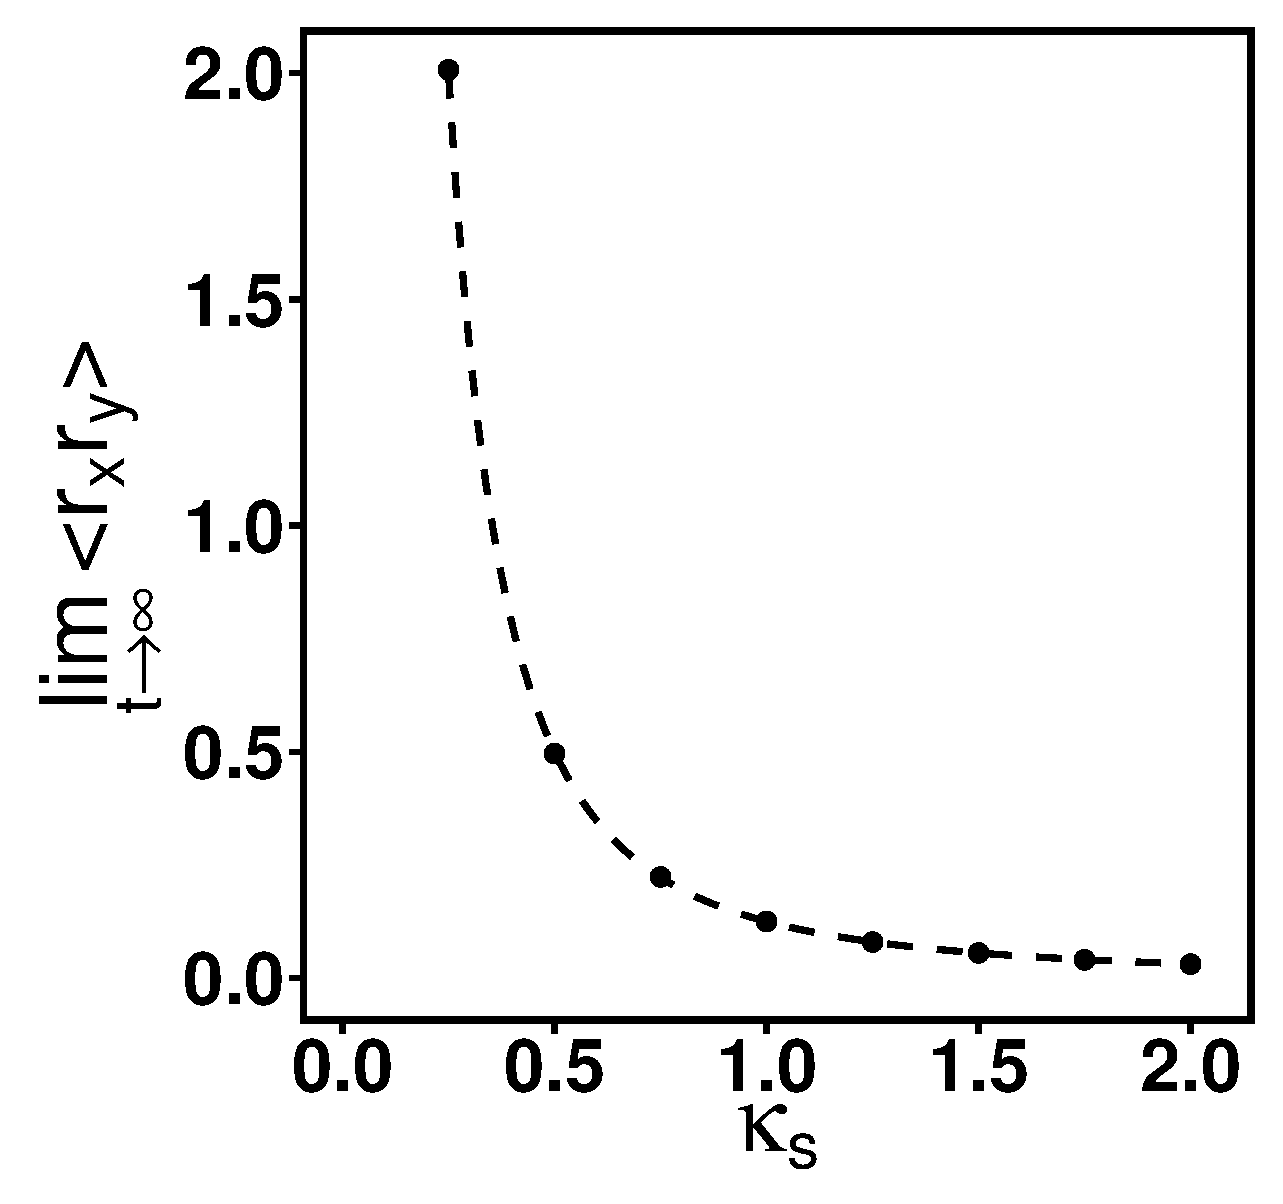
\includegraphics[scale = 0.4]{Figures/shear2M.eps}
            \caption{From \cref{eq: Case for 2 Monomers - viscosity due to particles I,eq: Case for 2 Monomers - viscosity due to particles II} we get \cref{eq: Case for 2 Monomers - Viscoelasticity - plot equation} which we use to check the validity of our code. We place the two monomer chain at the origin and then, under shear, by tracking the position vector of the chain we get the value for $\langle r_x r_y \rangle$ after a considerable amount of time. This can be plotted as a function of the spring constant of the chain, $\kappa_s$. We prove that the measurements extracted from our simulated system all fall under the dashed line representing \cref{eq: Case for 2 Monomers - Viscoelasticity - plot equation}. Parameters used: $g = 1$, $\Dot{\gamma} = 1$.}
            \label{fig: shear2M}
        \end{figure}
%
%\subsubsection{Effect of polymer chain size}
\subsection{Effect of Polymer Chain Size}
%
    Consider now the role of the size of the polymer chain on the effective viscosity. We know that the motion of the $n$-th monomer can be determined by the following Langevin equation
        \begin{equation}
            0 = -\zeta \left( \frac{d\mathbf{R}_n}{dt} - \mathbf{u}(\mathbf{R}_n) \right) - \frac{\partial U_{\kappa_s}}{\partial \mathbf{R}_n} + \bm{\xi}_n \,,
        \end{equation}
    meaning that, for a monomer inside the chain, $n \in [2,\, N-1]$,
        \begin{equation}\label{eq: Viscoelasticity - Langevin eq for a monomer inside the chain}
            \zeta\frac{d\mathbf{R}_n}{dt} = \zeta \Dot{\gamma} R_{n,y}\,\uvec{i} + \kappa_s\left( \mathbf{R}_{n+1} - 2\mathbf{R}_n + \mathbf{R}_{n-1} \right) + \bm{\xi}_n \,,
        \end{equation}
    whilst, for the extremities,
        \begin{align}
            \label{eq: Viscoelasticity - Langevin for extremities [1]}
            \zeta\frac{d\mathbf{R}_1}{dt} &= \zeta \Dot{\gamma} R_{1,y}\,\uvec{i} + \kappa_s\left( \mathbf{R}_{2} -\mathbf{R}_{1} \right) + \bm{\xi}_1 \,, \\
            \label{eq: Viscoelasticity - Langevin for extremities [2]}
            \zeta\frac{d\mathbf{R}_N}{dt} &= \zeta \Dot{\gamma} R_{N,y}\,\uvec{i} - \kappa_s\left( \mathbf{R}_N - \mathbf{R}_{N-1} \right) + \bm{\xi}_N \,.
        \end{align}
    Taking $\mathbf{R}_{0} = \mathbf{R}_{1}$ and $\mathbf{R}_{N+1} = \mathbf{R}_{N}$ allows us to write \cref{eq: Viscoelasticity - Langevin for extremities [1],eq: Viscoelasticity - Langevin for extremities [2]} as \cref{eq: Viscoelasticity - Langevin eq for a monomer inside the chain}. Making use of the bond vector definition (\cref{eq: Gaussian Chain - Bond Vector Definition}), we can further simplify \cref{eq: Viscoelasticity - Langevin eq for a monomer inside the chain} to
        \begin{equation}\label{eq: Viscoelasticity - Langevin eq for the bond vector}
            \zeta\frac{d\mathbf{r}_n}{dt} = \zeta \Dot{\gamma} r_{n,y}\uvec{i} + \kappa_s\left( \mathbf{r}_{n+1} - 2\mathbf{r}_n + \mathbf{r}_{n-1} \right) + \bm{\Xi}_n \,,
        \end{equation}
    which now holds for $n \in [1,\, N]$.
    
    From numerical implementation of our Gaussian chain model, we show in \cref{fig: shear - chain size}, that $\eta^{(p)}$ scales with $N^2$, just as predicted in the literature \cite{doiTheoryPolymerDynamics1988}. Since we kept $\Dot{\gamma} = 1$, the value for $\eta^{(p)}$ is given by the stress tensor, $\sigma_{xy}$, calculated in the final iterations of our simulated system [\cref{eq: Viscoelasticity - stress tensor due to solvent}].
        \begin{figure}[h]
            \centering
            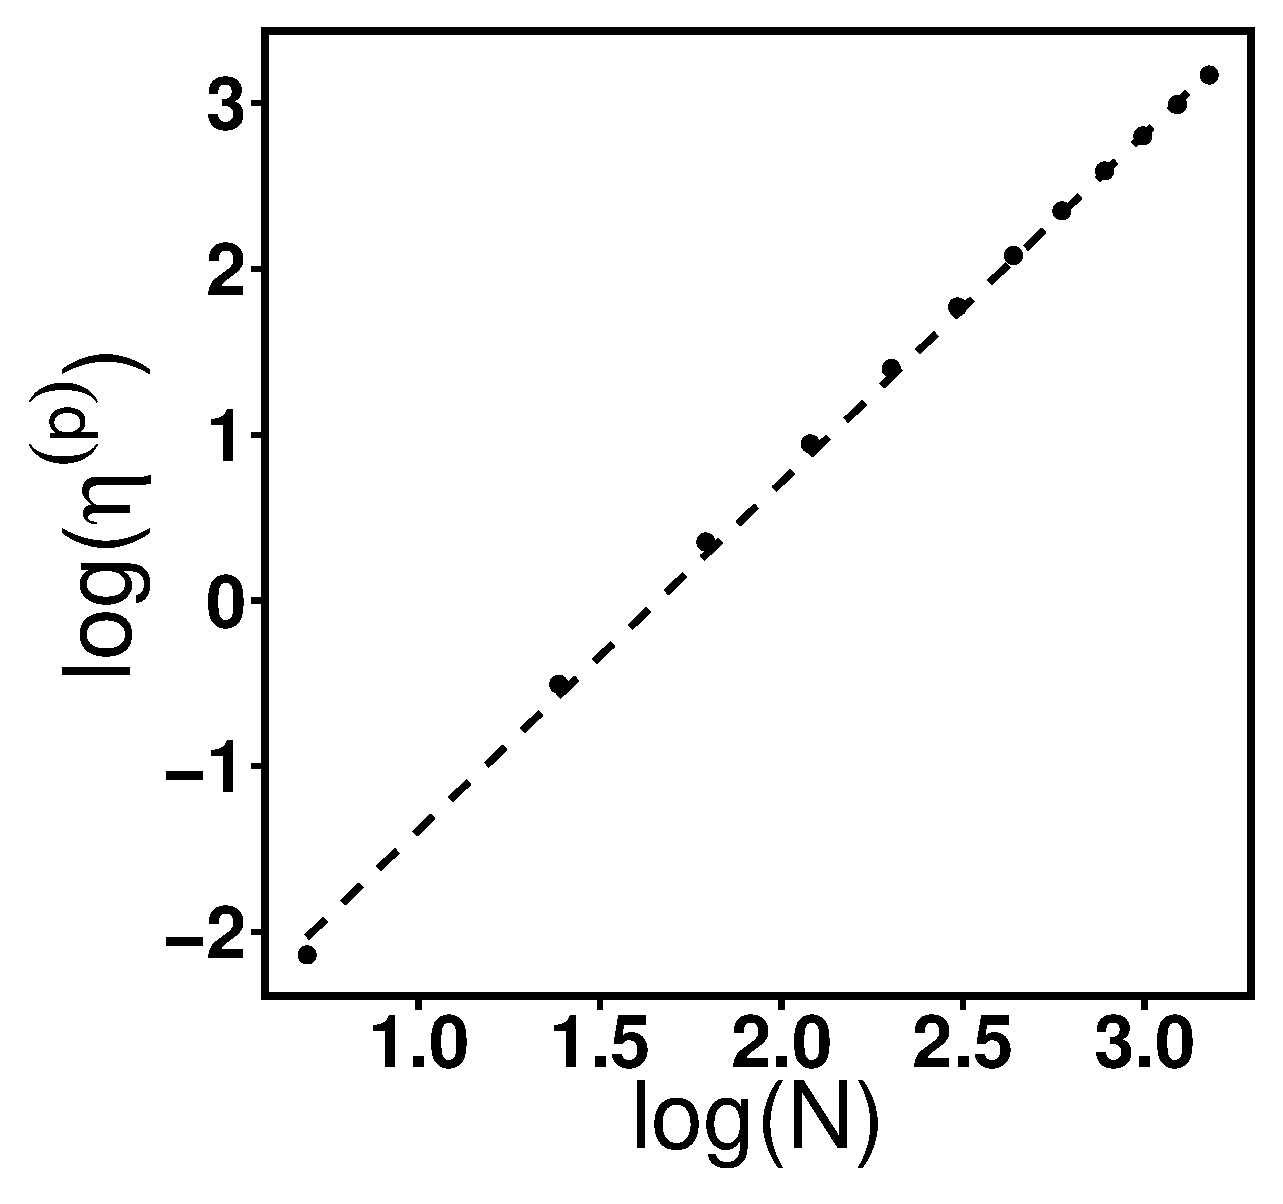
\includegraphics[scale=0.4]{Figures/shear_Nchains.eps}
            \caption{By taking a log-log plot of the viscosity due to the particles, $\eta^{(p)}$, in relation to the chain size, $N$, we show that there is a power law relation. The dashed line, whose slope is $\approx2$, represents the linear regression of the points obtained through numerical simulation. Parameters used: $g = 1$, $\Dot{\gamma} = 1$.}
            \label{fig: shear - chain size}
        \end{figure}
       
%
\end{document}